
\section*{Problema P6.2}

\renewcommand*\thesection{6.2}
\numberwithin{equation}{section}

\begin{center}
    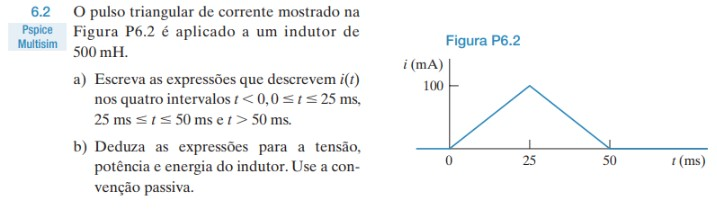
\includegraphics[scale=1.0]{P6.2.jpg}
\end{center}

\subsection*{(a)}

Usando a figura, temos as expressões de $i(t)$ dadas por

\[ i(t) =
    \begin{cases}
        0,                                                                    & t < 0                 \\
        \noalign{\vskip9pt}
        \frac{100 \cdot 10^{-3} - 0}{25 \cdot 10^{-3} - 0}\;t,                & 0 \leq t < 25 \un{ms} \\
        \noalign{\vskip9pt}
        \frac{0 - 100 \cdot 10^{-3}}{50 \cdot 10^{-3} - 25 \cdot 10^{-3}}\;t + (200 \cdot 10^{-3}), & 25 \leq t < 50 \un{ms} \\
        \noalign{\vskip9pt}
        0,                                                                    & t \geq 50 \un{ms}
    \end{cases}
    =
    \begin{cases}
        0 \un{A},   & t < 0                 \\
        \noalign{\vskip9pt}
        4t \un{A},  & 0 \leq t < 25 \un{ms} \\
        \noalign{\vskip9pt}
        0.2 - 4t \un{A}, & 25 \leq t < 50 \un{ms} \\
        \noalign{\vskip9pt}
        0 \un{A},   & t \geq 50 \un{ms}
    \end{cases}
\]

\subsection*{(b)}

Sabemos que a tensão em um indutor é dada por   

\begin{equation}\label{eq:6.2.1}
    v(t) = L\diff{i}{t}
\end{equation}

Portanto, aplicando \eqref{eq:6.2.1} sobre o resultado do item (a), temos

\[ v(t) =
    \begin{cases}
        0,   & t < 0                 \\
        \noalign{\vskip9pt}
        L \cdot 4,  & 0 \leq t < 25 \un{ms} \\
        \noalign{\vskip9pt}
        L \cdot (-4), & 25 \leq t < 50 \un{ms} \\
        \noalign{\vskip9pt}
        0,   & t \geq 50 \un{ms}
    \end{cases}
    =
    \begin{cases}
        0 \un{V},   & t < 0                 \\
        \noalign{\vskip9pt}
        2 \un{V},  & 0 \leq t < 25 \un{ms} \\
        \noalign{\vskip9pt}
        -2 \un{V}, & 25 \leq t < 50 \un{ms} \\
        \noalign{\vskip9pt}
        0 \un{V},   & t \geq 50 \un{ms}
    \end{cases}
\]

Além disso, temos que a potência no indutor é dada por   

\begin{equation}\label{eq:6.2.2}
    p(t) = v(t) \cdot i(t)
\end{equation}

Assim,

\[ p(t) =
    \begin{cases}
        0,   & t < 0                 \\
        \noalign{\vskip9pt}
        4t \cdot 2,  & 0 \leq t < 25 \un{ms} \\
        \noalign{\vskip9pt}
        (0.2 - 4t)\cdot (-2), & 25 \leq t < 50 \un{ms} \\
        \noalign{\vskip9pt}
        0,   & t \geq 50 \un{ms}
    \end{cases}
    =
    \begin{cases}
        0 \un{W},   & t < 0                 \\
        \noalign{\vskip9pt}
        8t \un{W},  & 0 \leq t < 25 \un{ms} \\
        \noalign{\vskip9pt}
        8t - 0.4 \un{W}, & 25 \leq t < 50 \un{ms} \\
        \noalign{\vskip9pt}
        0 \un{W},   & t \geq 50 \un{ms}
    \end{cases}
\]

Finalmente, podemos determinar a energia $E(t)$ no indutor a partir de $p(t)$ substituindo \eqref{eq:6.2.1} em \eqref{eq:6.2.2}.

\[ p(t) = L\diff{i}{t} \cdot i(t) = L\;i(t)\diff{i}{t}  \]

Note que a potência é energia por unidade de tempo, logo $p(t) = \diff{E}{t}$. Substituindo,

\[ \diff{E}{t} = L\;i(t)\diff{i}{t}  \]

\[ dE = L\;i(t)di  \]

Integrando ambos lados, temos

\[ \int_{t_i}^{t_f} E(t) \,dt = \int_{i_i}^{i_f} Li(t) \,di  \]

\[ E(t_f) - E(t_i) = \frac{1}{2}L\left[i_f^2 - i_i^2\right]  \]

Assumimos a corrente inicial $i_i =0$ e energia inicial $E_i = 0$ também nula. Além disso, fazemos
a energia final $E(t_f) = E(t)$ e a corrente do estado final como $i_f = i(t)$. Assim, isolando $E(t)$,

\begin{equation}\label{eq:6.2.3}
    E(t) = \frac{1}{2}L\left[i(t)\right]^2
\end{equation}

Usando \eqref{eq:6.2.3}, temos 

\[ E(t) =
    \begin{cases}
        0,   & t < 0                 \\
        \noalign{\vskip9pt}
        \frac{1}{2}L(4t)^2,  & 0 \leq t < 25 \un{ms} \\
        \noalign{\vskip9pt}
        \frac{1}{2}L(0.2 - 4t)^2, & 25 \leq t < 50 \un{ms} \\
        \noalign{\vskip9pt}
        0,   & t \geq 50 \un{ms}
    \end{cases}
    =
    \begin{cases}
        0 \un{J},   & t < 0                 \\
        \noalign{\vskip9pt}
        4t^2 \un{J},  & 0 \leq t < 25 \un{ms} \\
        \noalign{\vskip9pt}
        0.01 - 0.4t + 4t^2 \un{J}, & 25 \leq t < 50 \un{ms} \\
        \noalign{\vskip9pt}
        0 \un{J},   & t \geq 50 \un{ms}
    \end{cases}
\]





